\documentclass[../Bachelorarbeit.tex]{subfiles}
\begin{document}

\graphicspath{{./figures/theory/}}	%specifying the folder for the figures

\chapter{Theory}
\label{ch:theory}

In this chapter the theory necessary to understand the fundamentals of the thesis is covered. 

TODO: der theorie-teil. Soll in die verwendete Theorie des Hauptteils einführen und darauf hinweisen, aber nicht völlig trocken und losgelöst vom hauptteil sein. Soll immer den kontext des hauptteils berücksichtigen und schon gewisse anwendungsfälle vorwegnehmen.

TODO: jeden abschnitt erklären, wieso er notwendig ist bzw. auf was er in der restlichen thesis hinweist 

\section{Equilibrium Theory}

Clearing of prices.
	
\paragraph{Clearing}
In equilibrium theory clearing is the process of finding a price in which all demands are matched to the given supplies thus clearing the market by leaving no unmatched demands or supplies. In other words it tries to find a price which satisfies all offers.

\begin{figure}[H]
	\centering
  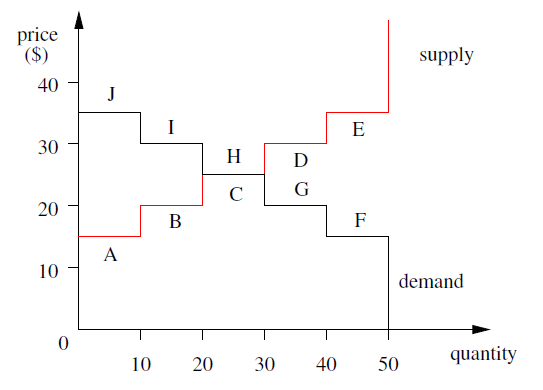
\includegraphics[width=1.0\textwidth, angle=0]{CLEARING.png}
  	\caption{Illustrative supply and demand curves for a double auction. Diagram taken from \cite{Parsons2006}}
	\label{fig:CLEARING}
\end{figure}

In this diagram the equilibrium price which clears the market would be at 25\$ because this price satisfies the constraint buyer-price $\geq$ seller-price for all traders, thus all traders match and the market is cleared. The constraint buyer-price $\geq$ seller-price is a fundamental law of economics and imposes an ordering on the prices of the market and is rooted in the fact that a buyer values the good it wants to buy more than the seller and has to pay at least the amount of money the seller wants for it, or more. TODO: irgendwie belegen


TODO: notwendig für das model in geanakoplos: welche equilibrium-berechnungen stehen hinter dem model von ihm?
preise p werden festgelegt und traders maximieren ihre utility.
WIKI: general equilibrium theory

WIKI:
-> 2 common notions of equilibrium exist: walrasian- and price-equilibrium with transfers


\subfile{./tex/DoubleAuctionTheory.tex}

\section{Systemic Risk}
TODO: auslassen, ist ein gigantisches und extrem komplexes thema und hat nur ganz abstrakt etwas mit der thesis zu tun. WENN NOCH ZEIT: Market Dynamics and Systemic Risk lesen und falls es etwas konkretes mit der thesis zu tun hat.

WIKI: It refers to the risks imposed by interlinkages and interdependencies in a system or market, where the failure of a single entity or cluster of entities can cause a cascading failure, which could potentially bankrupt or bring down the entire system or market.

\cite{Milan2010}

\section{Leverage}
TODO: im geanakoplos-paper seite 1

WIKI: In finance, leverage (sometimes referred to as gearing in the United Kingdom and Australia) is any technique to multiply gains and losses.

Accounting Leverage
Notational Leverage
Economic Leverage

Systemic risk and leverage are tightly coupled in a way that leverage increases systemic risk dramatically as was the case in the "Subprime Mortgage Crisis".

TODO: leverage in housing market and its dangers to create bubbles (the leverage cycle).

\section{Complex Networks}
\label{sec:theory_complexNetworks}
small-world
power-law distribution
generation algorithms
dient hauptsächlich zur kategorisierung
		
TODO:
In "State of the art" an overview of abstract networks and their properties is given. Also network-generating algorithms are presented and discussed. Because continuous double-auctions are the type of market which is used for matchings a short introduction is given on this topic too.\\

TODO: ziel hier eine theoretische übersicht über  netzwerk-theorie zu geben wobei hauptaugenmerk auf die entwicklungen der letzten jahre (scale-free, small-world, ...)

Regular Graphs: \citep[vgl.]{BarabasiAlbert_StatisticalMechanics} \citep[vgl.]{Newman_ComplexNetworks}

Random Graphs: but since then, most large scale networks with no apparent design principle were described as random graphs introduced by two Hungarian mathematicians Paul Erdos and Alfred Renyi \citep[vgl.]{ErdosRenyi_RandomGraphs} \citep[vgl.]{ErdosRenyi_EvolutionRandomGraphs} Have small-world properties.

Small World Graphs or Average Path Length: Stanley Milgram \citep{TraverMilgram_StudySmallWorld} \citep{Milgram_SmallWorld} \citep{Kleinberg_SmallworldAlgorithmic}

Clustering Coefficient or Transitivity \citep{WattsStrogatz_DynamicsSmallWorld}

Degree Distribution \citep{BarabasiAlbert_EmergenceScaling} Generally, it was believed that the degree distribution in most networks follows a
Poisson distribution but in reality, real world networks have a highly skewed degree distribution following power-laws. Power-laws are expressions of the form y / x, where is a constant, x and y are the measures of interest [152].

Small World and Scale Free Network: A small world network as deined by Watts and Strogatz \cite{WattsStrogatz_DynamicsSmallWorld}, is a network with high clustering coeffcient and small average path length. A scale free network as deined by Barabasi and Albert \citep{BarabasiAlbert_EmergenceScaling}, is a network where the degree distribution follows a power law.

Complex Networks: are Small-World and/or Scale-Free \citep{BarratWeigt_PropertiesSmallWorld} \citep{AmaralScalaStanley_ClassesSmallWorld}

\citep {Kleinfeld_BigWorld}
http://www.cs.princeton.edu/~chazelle/courses/BIB/big-world.htm

introduce Metrics:
- Average degree
- average path-length
- average clustering coefficient
- network diameter
- graph density

Mathematical stuff 
\citep{Newman_Eigenvectors}
\citep{AielloChungLu_RandomEvolution}
\citep{EbelMielschBornholdt_TopologyEmail}
\citep{GaertlerPatrignani_AutonomousSystem}

\subsection{Network-Generating Algorithms}
- fully connected
- ascending connected
- ascending connected with shortcuts
- hubs
- erdos-renyi
- barbasi-albert
- watts-strogatz

TODO: reference to appendix a for concrete pictures of topologies

\end{document}